\documentclass[12pt]{article}
\usepackage{amsmath,amssymb,amsthm}
\usepackage{graphicx}
\usepackage{subcaption}
\usepackage{float}
\PassOptionsToPackage{hyphens}{url}\usepackage{hyperref}\usepackage{color}
\usepackage{enumitem}
\usepackage{tabularx}
\usepackage[sorting=none]{biblatex}
\usepackage[raggedrightboxes]{ragged2e}
\setlength{\headheight}{15pt}
\usepackage{fancyhdr}

\usepackage[table,xcdraw]{xcolor}
\usepackage[normalem]{ulem}
\useunder{\uline}{\ul}{}


% figure and bibliography source
\addbibresource{../prime-editing.bib}
% add figure path
\graphicspath{ {../figures/} }
% reduce margin
\usepackage[margin=1in]{geometry}
% increase title font size
\usepackage{titling}
\pretitle{\begin{center}\Huge\bfseries}

\pagestyle{fancy}


\setlist[enumerate]{itemsep=0mm}


\title{Surveying Machine Learning Methods for Predicting the Outcomes of \newline Prime Editing}
\author{1592800}
\fancyfoot[R]{1592800}

\begin{document}
\date{April, 2024}
\maketitle


\newpage



%table of contents
\tableofcontents



\newpage


\section{Background and Introduction}

Genome editing is a powerful tool for understanding the genetic basis of life and for developing new therapies. The ability to precisely edit the genome of living organisms has been a long-standing goal of genetic engineering and inspired the development of various technologies. 

The discovery of CRISPR(Clustered Regularly Interspaced Short Palindromic Repeats) and its associated family of Cas9 proteins revolutionized the field of genetic engineering. CRISPR-Cas9 is an adaptive prokaryotic immune system that detects invading viruses and plasmids, and damages their gene sequences. It was harnessed by researchers to provide a precise method for editing the genome of living organisms, leveraging its ability to recognize specific gene sequences and produce scission\cite{jiangCRISPRCas9Structures2017}. A number of CRISPR-Cas9 based tools have been developed since the discovery of the original system, including CRISPR-Cas9 HDR(Homology Directed Repair), base editors, and prime editors.

\begin{figure}[ht]
    \centering
    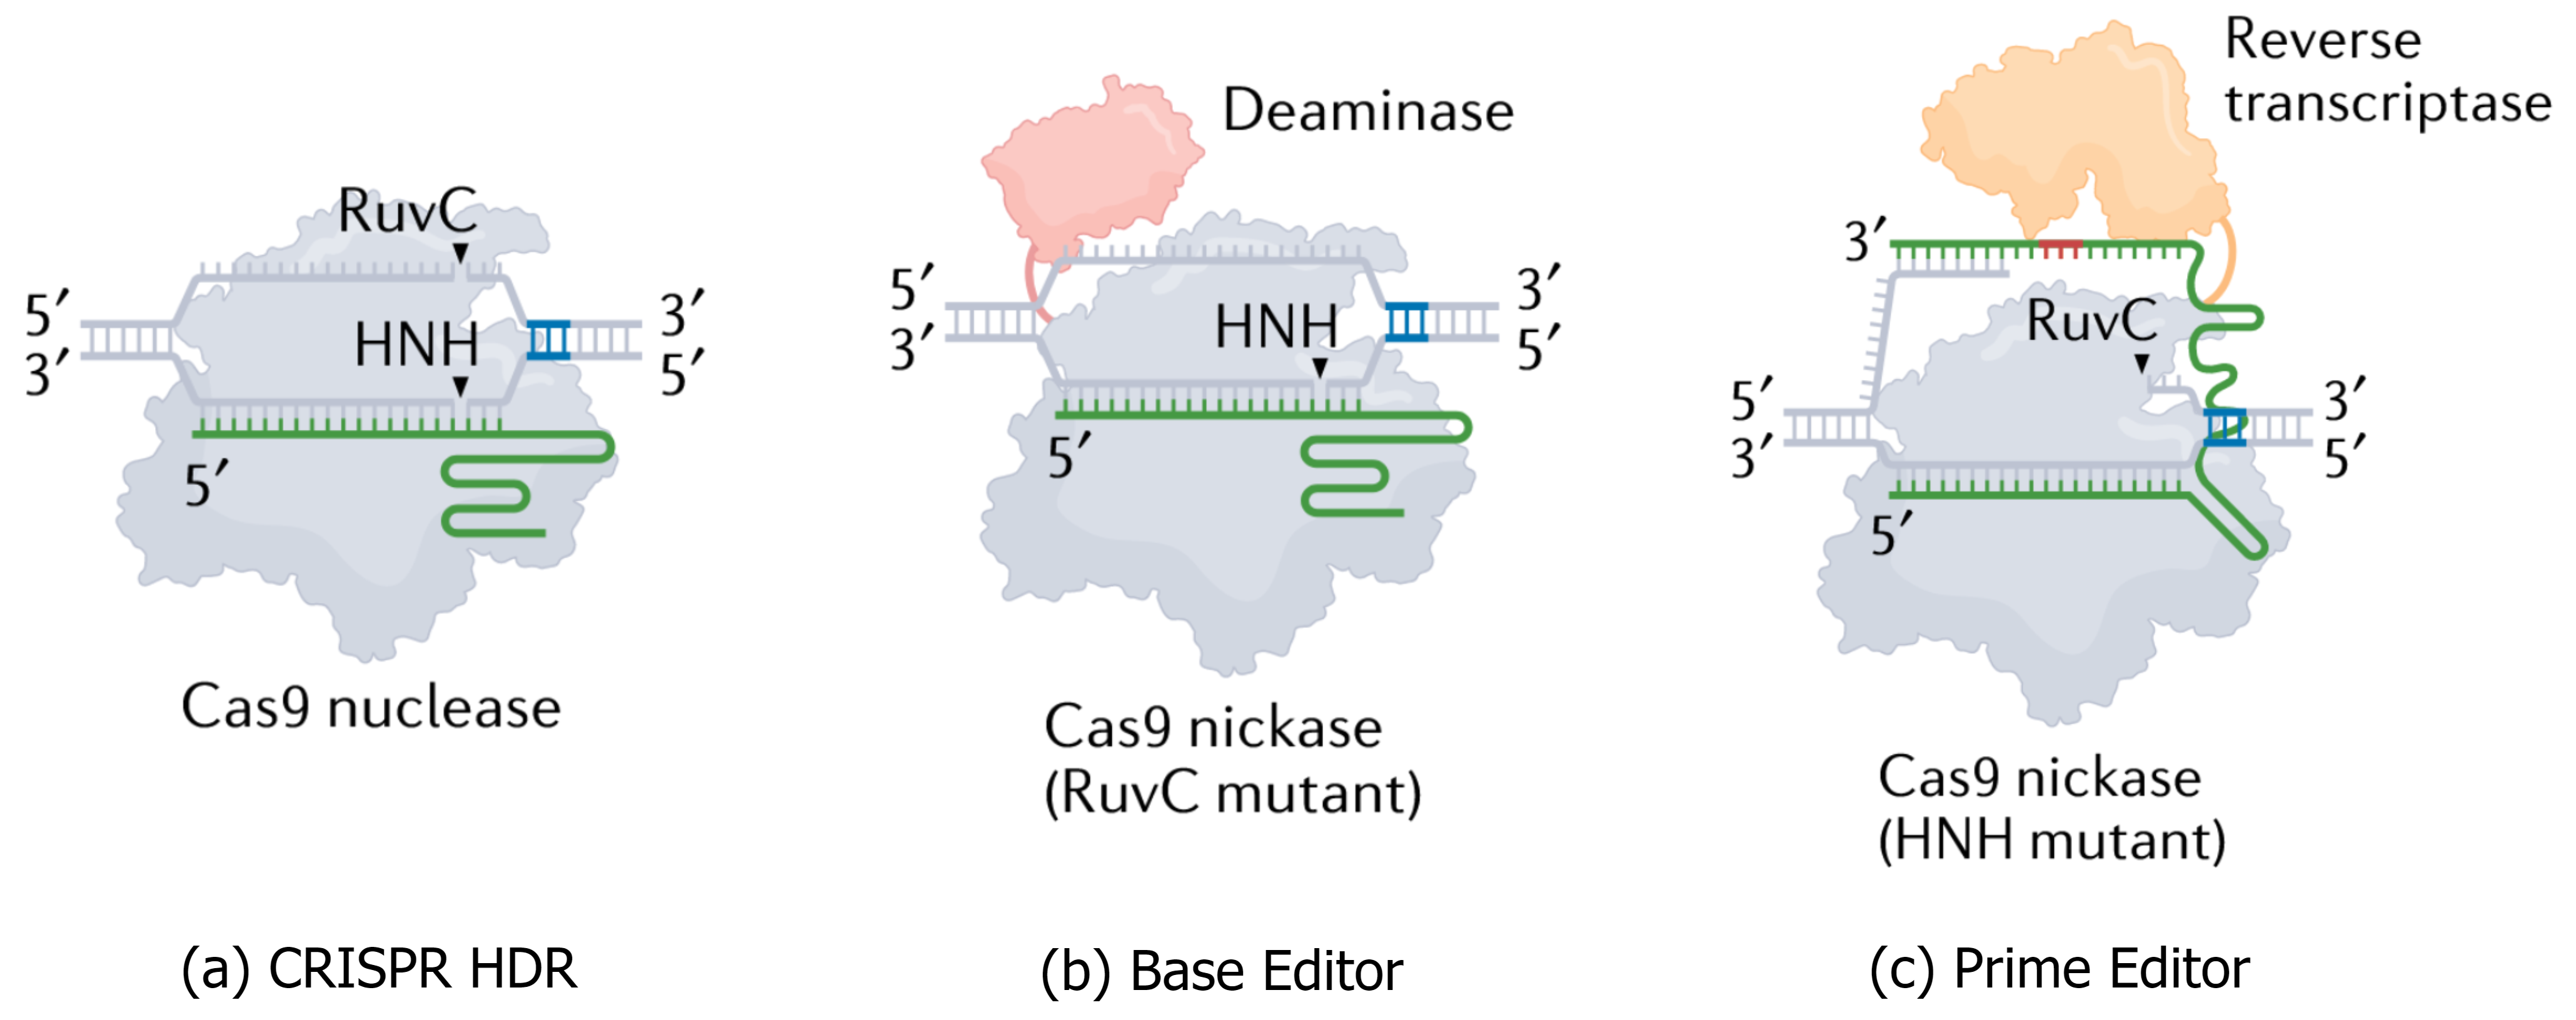
\includegraphics[width=0.9\textwidth]{hdr-base-prime-editors.png}
    \caption{Structure of CRISPR-Cas9, Base Editors, and Prime Editors\cite{liuPrimeEditingPrecise2023}}
    \label{fig:editors}
\end{figure}

\subsection{CRISPR-Cas9 HDR}


Shown in \autoref{fig:editors} (a), the CRISPR-Cas9 system consists of two components: a single guide RNA(sgRNA) that binds to a target DNA sequence(the protospacer) complementary to the sgRNA, and a Cas9 protein that cuts both strands of the DNA at the target site. To install intended edits, an exogenous DNA template is also provided to the cell. The cell's endogenous repair pathway Homology Directed Repair(HDR) can then uses the template to repair the broken DNA sequence, resulting in the desired edit.

However, a competing repair pathway, Non-Homologous End Joining (NHEJ), is the preferred pathway in many cell types and can introduce unwanted insertions and deletions (indels) at the cut site. This can lead to undesirable effects and limit the therapeutic potential of CRISPR-Cas9 HDR system. As a result, CRISPR-Cas9 HDR is now mostly used for the disruption of the target genome instead of precise editing\cite{kantorCRISPRCas9DNABaseEditing2020}. 

\subsection{Base Editors}

Developed by David R. Liu and colleagues, base editors eliminate the involvement of NHEJ by directly converting one base pair to another without introducing a double-strand break (DSB). The components of a typical base editor are shown in \autoref{fig:editors} (b). The system consists of a Cas9 nickase fused to a deaminase enzyme that converts a base pair to another, and a sgRNA that binds to the protospacer. The Cas9 nickase nicks the DNA strand complementary to the sgRNA at target location, then the deaminase enzyme chemically converts the target base pair. Finally, the cell's endogenous repair system repairs the nicked DNA strand using the modified strand as template, installing the desired edit into the genome\cite{reesBaseEditingPrecision2018}.

The base editors significantly increased the editing efficiency and reduced the off-target effects compared to the CRISPR-Cas9 HDR system. However, limited by the deaminase enzyme, base editors can only introduce point mutations. Additionally, most base editors can only introduce transition mutations(A-T$\iff$G-C) and not transversion mutations(G-C$\iff$C-G, A-T$\iff$T-A), further limiting their viabilities\cite{kantorCRISPRCas9DNABaseEditing2020}.

\subsection{Prime Editors}

Determined to fix the limitations of CRISPR HDR and base editors, David R. Liu and colleagues developed prime editors, a new class of genetic editing tools that can introduce a wide range of edits, including varying lengths of insertions and deletions. \autoref{fig:editors} (c) shows the structure of a prime editor. 

The system consists of a SpCas9 nickase fused to a reverse transcriptase and a prime editing guide RNA(pegRNA). The pegRNA is similar to sgRNA used in CRISPR-Cas9 and base editors at its $5'$ ends(and thus this section will be referred to as sgRNA in the rest of the survey), but is extended in its $3'$ end to include a prime binding site(PBS) and a reverse transcriptase template(RTT) complementary to the desired edit. The two functional ends are connected together with a tracrRNA scaffolding sequence that should have no significant effects during the editing process.

\begin{figure}[ht]
    \centering
    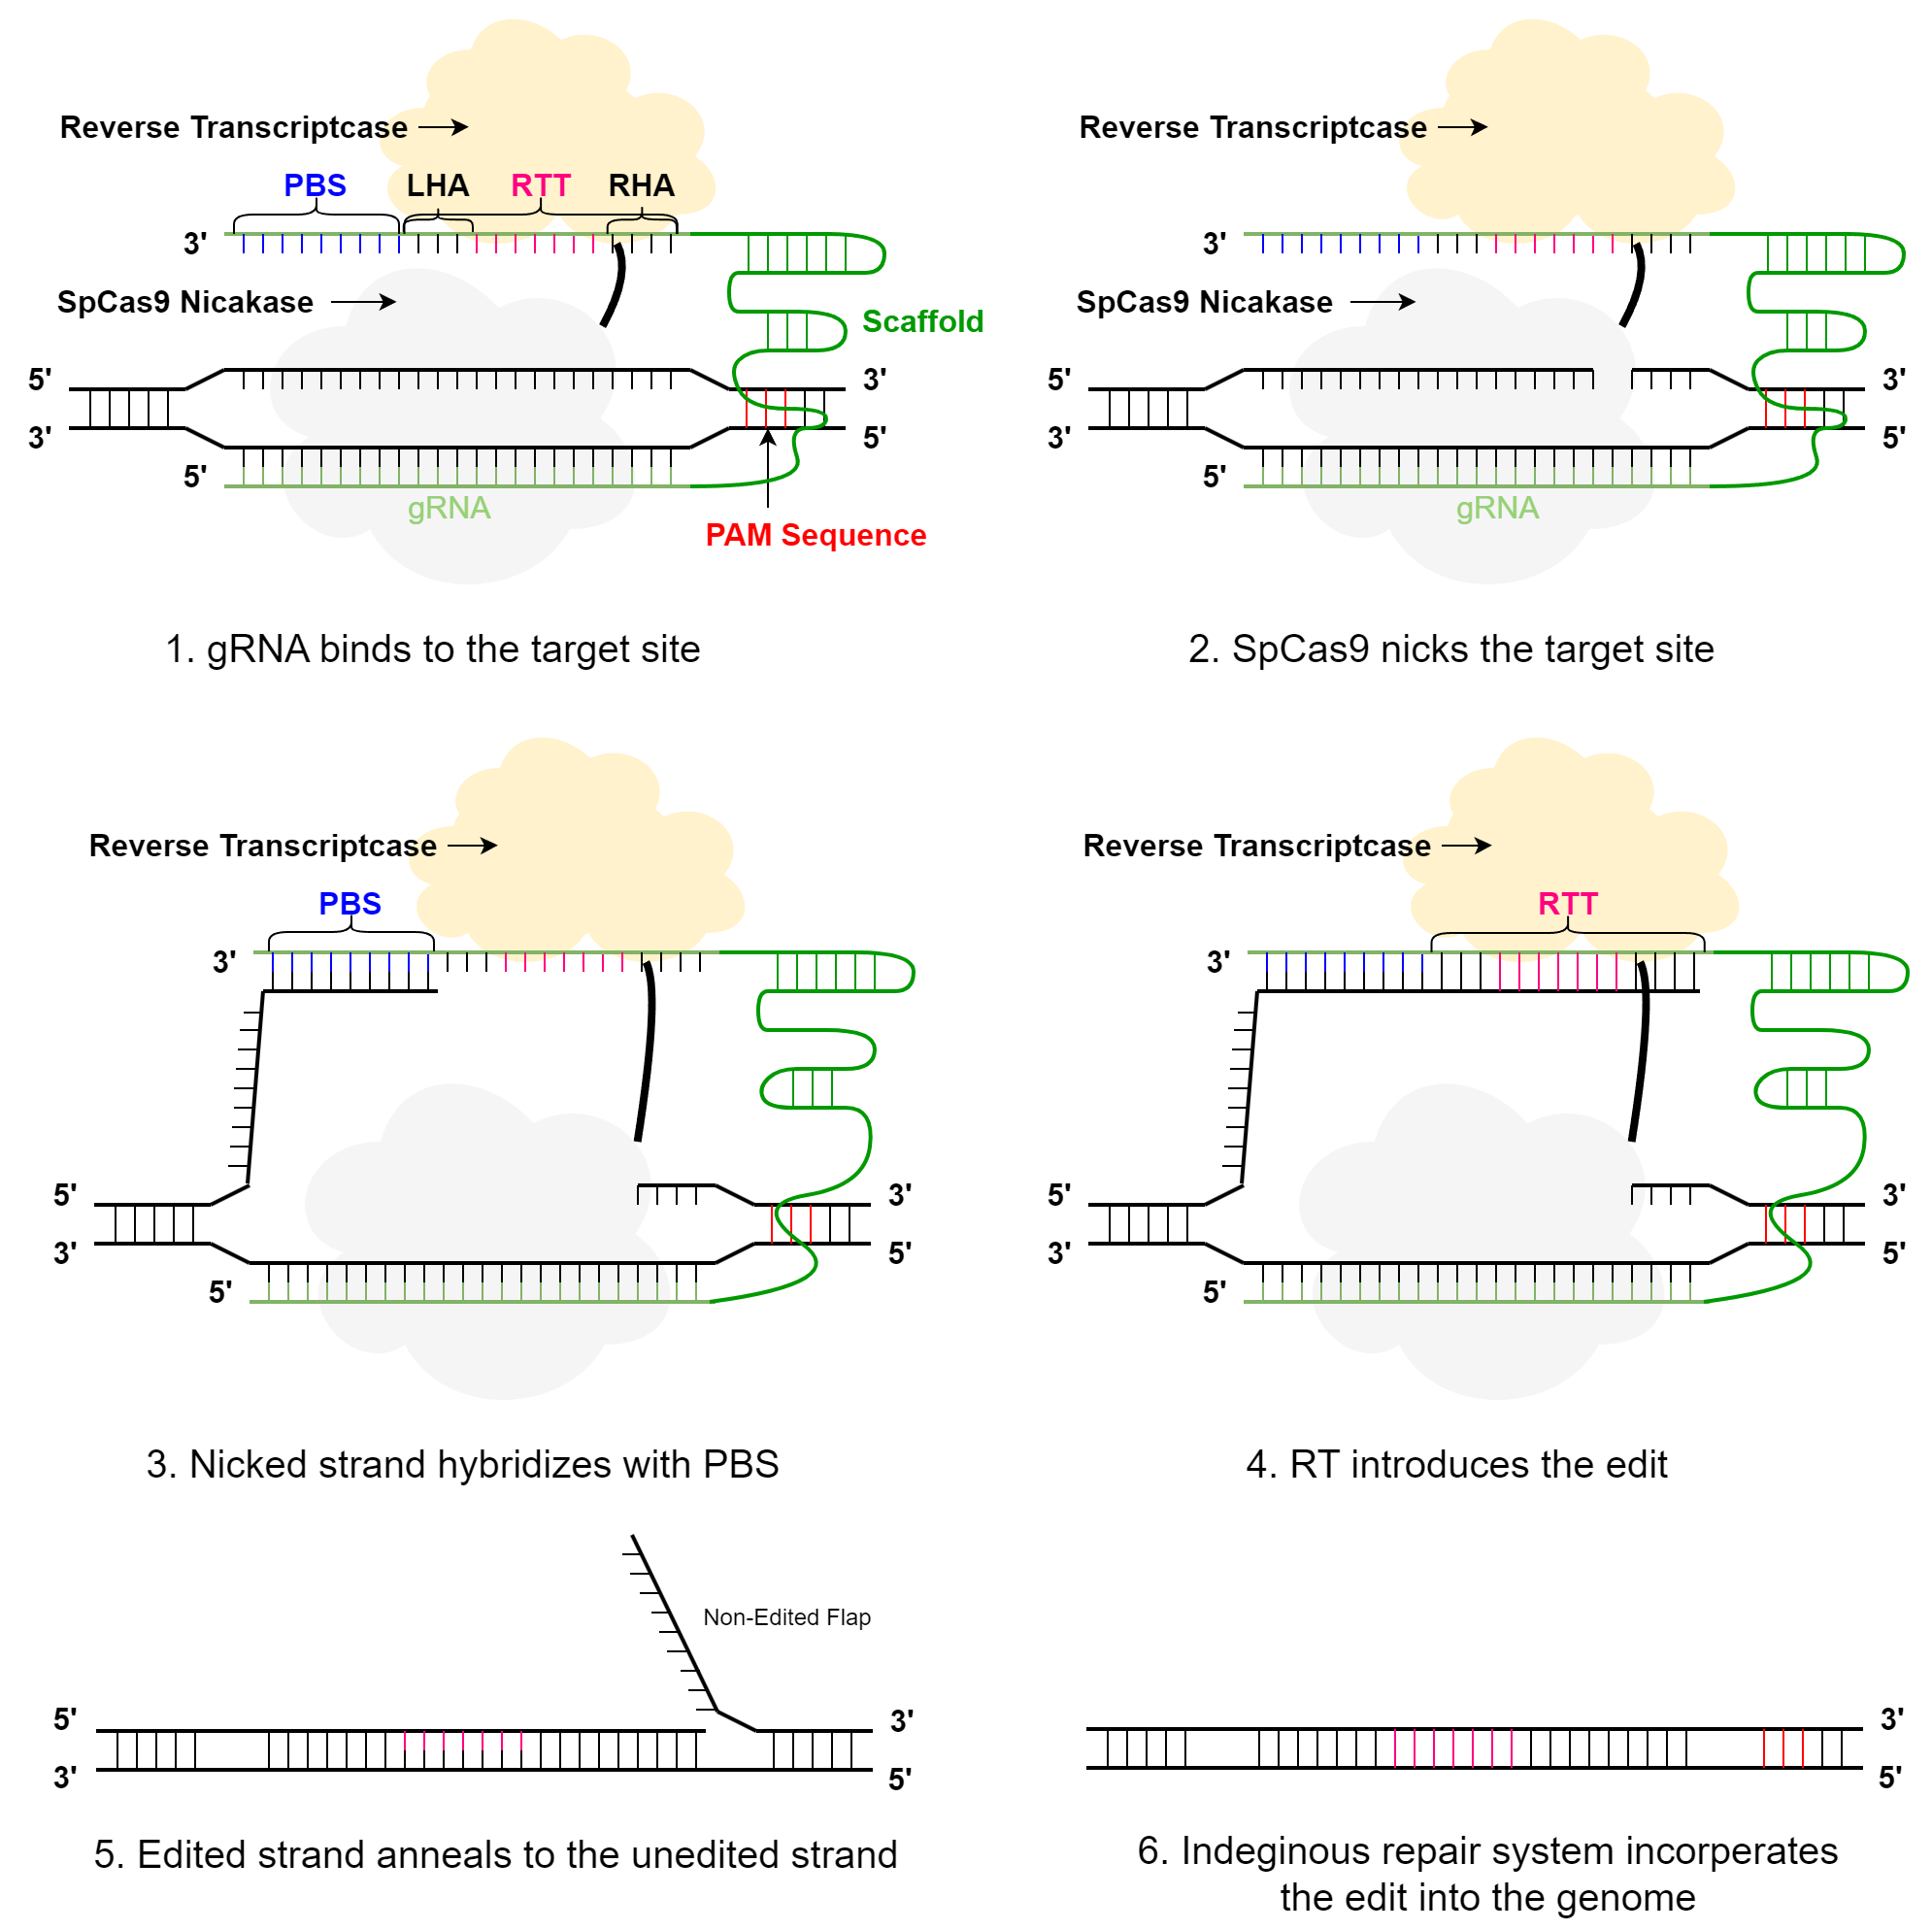
\includegraphics[width=0.9\textwidth]{prime-editing-process.png}
    \caption{Prime Editing Process\cite{liuPrimeEditingPrecise2023}}
    \label{fig:prime-editing}
\end{figure}

The prime editing process is a multi-stage procedure consisting of\cite{liudavidr.SearchandreplaceGenomeEditing2019}:
\begin{enumerate}
    \item The sgRNA at the $5'$ end of pegRNA binds to the protospacer, then the Cas9 nickase introduces a scission in the exposed strand.
    \item The PBS at the $3'$ end of pegRNA binds to the now displaced strand.
    \item The reverse transcriptase introduces the edits according to the template provided.
    \item The edited strand hybridizes with the non-edited stand, reforming the double helix.
    \item The cell's endogenous repair system installs the edits into the non-edited strand, permanently adding the modification into the genome.
\end{enumerate}

The first three steps of the process are illustrated in \autoref{fig:prime-editing}. 


This concludes the editing process for prime editors PE1 and PE2, where PE2 is the much more efficient version of PE1 using a different reverse transcriptase\cite{liudavidr.SearchandreplaceGenomeEditing2019}. 
The more efficient PE3 includes an extra ngRNA(nicking guide RNA) that introduces a nick in the non-edited strand to encourage the cell's DNA repair system to use the edited strand as the template\cite{liudavidr.SearchandreplaceGenomeEditing2019}. 

More advanced versions of the prime editors have been developed after the publication of the original prime editors(PE1-PE3), two important examples are PE4 and PE5. PE4 and PE5 are the results of combining an additional MLH1dn protein with the original PE2 and PE3 respectively. 

The MLH1dn protein is a dominant negative mutant of the human MutL homolog 1(MLH1) protein, which is involved in the mismatch repair pathway(MMR). MMR can revert the nicked heteroduplex formed when the edited $3'$ DNA flap anneals to the genome in the final step, reducing editing efficiency when the edits produce mismatches known to be repaired by MMR. 

The edits repairable by MMR include single base substitution as well as short sequence insertion or deletion. The MLH1dn protein inhibits MMR activities shown to antagonize the prime editing efficiency in those cases,  increasing the overall editing efficiency of the prime editors\cite{chenEnhancedPrimeEditing2021}.

\subsection{pegRNA Design}

For all versions of the prime editors, the design of pegRNA is the most crucial step of the editing process. Performing the same edit on the same target sequence with different pegRNAs can result in different editing efficiencies. However, the experimental process of testing the efficiency of different pegRNAs on a specific target sequence is laborious and expensive, significantly limiting the therapeutic potential of prime editing\cite{mathisPredictingPrimeEditing2023}. 

A number of in silico methods have thus been developed, using the hardcoded design guideline suggested by the Liu lab to recommend a number of pegRNA sequences for a given target sequence\cite{hwangPEDesignerPEAnalyzerWebbased2021}. However, how to unbiasedly optimize the combination of the features from the design guide and identify the most suitable sequence from a list of candidates remains problematic\cite{liEasyPrimeMachineLearning2021}. 

pegRNA design has the additional challenge of prime editing being a multi-stage process. The resulting sequence of each stage will have an impact on the efficiencies of the subsequent stages, creating a significantly larger search space for the traditional optimization methods when compared to less complex methods such as base editing.

These problems inspired a cohort of researchers to apply machine learning methods to predict the outcomes of prime editing using a given pegRNA, leveraging a number of known determinants of prime editing efficiency as well as the pattern finding capabilities of machine learning algorithms. This survey aims to review the methods currently available and to identify new opportunities in the field.

\section{Methods For pegRNA Design}

\subsection{Determinants of Prime Editing Efficiency}

Although the exact determinants of prime editing efficiency are not known to us due to the complex nature of prime editors\cite{mathisPredictingPrimeEditing2023}, high throughput screening from a number of studies have revealed a number of features that have strong correlation with the efficiencies of prime editing\cite{mathisPredictingPrimeEditing2023,yuPredictionEfficienciesDiverse2023,kimPredictingEfficiencyPrime2021a,koeppelPredictionPrimeEditing2023,chenEnhancedPrimeEditing2021}. I hereby summarize the findings of these studies for better understanding of the machine learning methods that may utilize them in their models.

\subsubsection{Prime Editor Features}

The composition of each component of the prime editor as well as the mutations to install(indicated by the RTT) will clearly have an impact on the efficiency of the editing process. Specifically, the features that have been found to be correlated with the editing efficiency include:

\begin{enumerate}
    \item \textbf{RHA Length}: The right homology arm(RHA) is the section of RTT after all the edits(starting from the $3'$ end), complementary to the non-edited strand. They help the edited strand hybridize with the non-edited strand, increasing the success rate of the edits being installed into the genome. As a result, a RHA too short would result in a lower editing efficiency\cite{yuPredictionEfficienciesDiverse2023}.
    \item \textbf{pegRNA Secondary Structure}: It was shown that stronger secondary structure of the pegRNA homology arm can increase the editing efficiency\cite{koeppelPredictionPrimeEditing2023}.
    \item \textbf{GC Content and Melting Temperature of PBS}: Higher GC content and melting temperature of the PBS can increase the efficiency of the editing process\cite{yuPredictionEfficienciesDiverse2023} 
    \item \textbf{PAM Sequence Disruption}: The protospacer adjacent motif(PAM) is a short sequence that is required for the binding of the Cas9 protein to the target DNA downstream of the protospacer. The PAM sequences were shown as blue base pairs in \autoref{fig:editors} and \autoref{fig:prime-editing}. 
    
    The prime editors have the possibility of rebinding to the edited DNA sequence before the cellular repair mechanism installs the edits into both stands. This can lead to the introduction of unwanted edits. 
    
    The disruption of the PAM sequence can prevent the rebinding and thus improve the efficiency of the editing process\cite{liuPrimeEditingPrecise2023,kimPredictingEfficiencyPrime2021a,koeppelPredictionPrimeEditing2023}.

    \item \textbf{Length of Modifications to Insert}: As expected, substituting, deleting or inserting a longer sequence is more difficult and thus less efficient than a shorter sequence\cite{marquartPredictingBaseEditing2021}. The efficiency remains relatively consistent for up to 3-5 base pairs(bp), but starts to decrease after that\cite{yuPredictionEfficienciesDiverse2023}.
    
    \item \textbf{Prime Editor Type}: Obviously, the different versions of prime editors have different efficiencies due to whether beneficial components such as the MLH1dn protein and the extra ngRNA are included or not.
\end{enumerate}

\subsubsection{Target Sequence Features}

The exact composition of the target sequence(protospacer) itself also has a significant impact on the result of editing. The sequence features that have been found to be correlated with the editing efficiency include:

\begin{enumerate}
    \item \textbf{Poly-T sequences}: Consecutive A-T sequences in the protospacer can reduce the effiency of the editing process, as poly-U sequences in the spacer(gRNA) of the pegRNA are known to cause catalytic inactivation and backtracking of RNA polymerase III\cite{mathisPredictingPrimeEditing2023}.
    \item \textbf{GC Content}: Having G/C nucleotides directly flanking the target base pair during single base editing can increase the efficiency of the editing process\cite{mathisPredictingPrimeEditing2023}.
    \item \textbf{Single Nucleotide Composition}: The appearance of certain nucleotides at specific positions in the protospacer can significantly increase or decrease editing efficiency. Suppose that position 1 is the 20th base pair from the PAM sequence, a T at the 16th position can hamper PE efficiency, while a G at the 17th position can increase the efficiency\cite{kimPredictingEfficiencyPrime2021a}. This is consistent with previous results showing that these positions are important for Cas9 nickase activity\cite{doenchOptimizedSgRNADesign2016}.
\end{enumerate}



\subsubsection{Target Context Features}

The in vitro or in vivo editing process is not isolated, and the environment the editors work under should also be considered when making predictions on editing efficiencies. Examples of the context features are:

\begin{figure}[ht]
    \centering
    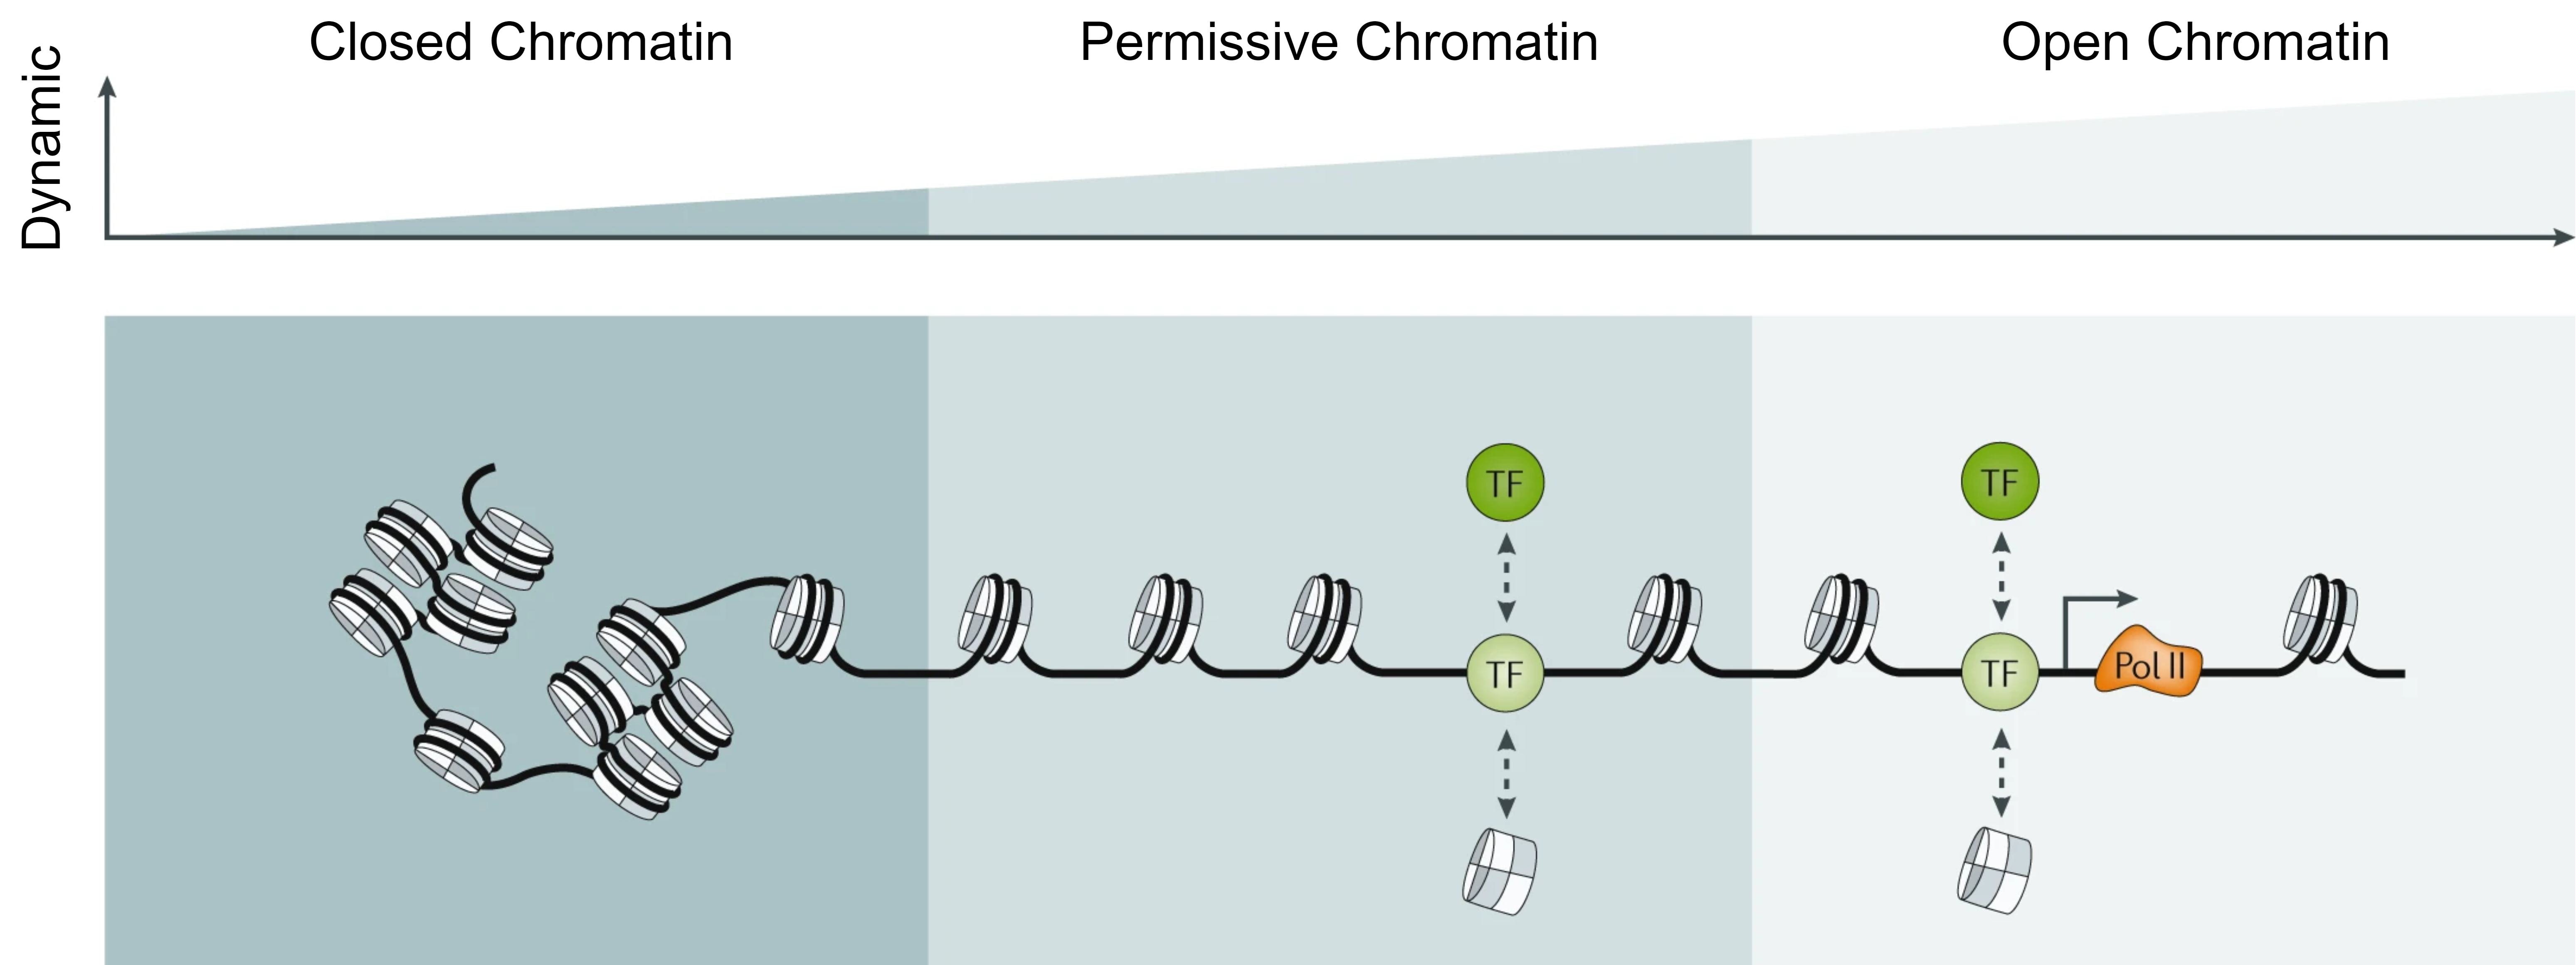
\includegraphics[width=\textwidth]{chromatin-accessibility.png}
    \caption{Levels of Chromatin Accessibility\cite{klemmChromatinAccessibilityRegulatory2019}}
    \label{fig:chromatin}
\end{figure}

\begin{enumerate}
    \item \textbf{Chromatin Accessibility of the Target Sequence}: The chromatin is the complex of DNA and proteins that make up the chromosomes in the Eukaryotic cells, such as the human embryonic kidney(HEK) cell lines often used in the experiments testing the capability of editors in human cells\cite{thomasHEK293CellLine2005}. Different levels of chromatin accessibility  are illustrated in \autoref{fig:chromatin}, where higher editing efficiency should be expected with more open chromatin\cite{mathisPredictingPrimeEditing2023}. 

    \item \textbf{Target Cell Type}: Different cell types used in the testing have different MMR activities. The HEK293T cell line is partly MMR deficient, while other cell lines such as HAP1(derived from a chronic myelogenous leukemia patient) are not. This results in PEs without the additional MLH1dn protein in PE4 and 5 having lower editing efficiency when doing short sequence substitution or insertion/deletion in the HAP1 cell line, compared to the HEK293T cell line\cite{koeppelPredictionPrimeEditing2023}.
\end{enumerate}

\subsection{Machine Learning Methods}
\label{sec:ml-methods}
\renewcommand{\arraystretch}{1.5}
\begin{table}
    \centering
    \begin{tabularx}{\textwidth}{p{0.14\textwidth}p{0.3\textwidth}p{0.25\textwidth}p{0.27\textwidth}}
        \textbf{Method}         & \textbf{Supported Cell Types}                                      & \textbf{Supported Edits}                                                                             & \textbf{Supported PEs}                                                                                                             \\
        \hline
        DeepPE         & HEK293T                                                   & G to C substitution at position +5 nick site & PE2                                                                                                                       \\
        EasyPrime     & HEK293T                                                   & GWAS Variants                                                                               & PE2, PE3, PE3b                                                                                                            \\
        MinsePIE       & HEK293T, HAP1                                              &      Insertion                                                                                       &        PE2, PE4                                                                                                                   \\
        DeepPrime(-FT) & HEK293T, HCT116, DLD1, MDA-MB-231, A549, HeLa, NIH3T3     & Substitution, Insertion, Deletion                                                           & PE2, PE2max, PE2max-e (PE2max with epegRNAs), PE4max, PE4max-e, NRCH-PE2, NRCH-PE2max, NRCH-PE4max \\
        PRIDICT        & HEK293T, K562, U2OS                                       & Substitution, Insertion, Deletion                                                           & PE2, PE2-max,PE3, PE3b, PE4                                                                                                         \\
        \hline
                       &                                                           &                                                                                             &                                                                                                                           \\
        \textbf{Method}         & \textbf{Code Availability}                                         & \textbf{Web Tool}                                                                                    & \textbf{Reference}                                                                                                                 \\
        \hline
        DeepPE         & \url{https://github.com/hkimlab-PE/PE\_SupplementaryCode} & \url{https://deepcrispr.info/DeepPE/}                                                       & \cite{kimPredictingEfficiencyPrime2021a}                                                                                  \\
        EasyPrime     & \url{https://github.com/YichaoOU/easy\_prime}             & \url{http://easy-prime.cc/}                                                                 & \cite{liEasyPrimeMachineLearning2021}                                                                                     \\
        MinsePIE       & \url{https://github.com/julianeweller/MinsePIE}           & \url{https://elixir.ut.ee/minsepie/}                                                        & \cite{koeppelPredictionPrimeEditing2023}                                                                                  \\
        DeepPrime(-FT)                  & \url{https://github.com/hkimlab/DeepPrime}      & \url{https://deepcrispr.info/DeepPrime/}                                             & \cite{yuPredictionEfficienciesDiverse2023}                                                                                \\
        PRIDICT        & \url{https://github.com/uzh-dqbm-cmi/PRIDICT}             & \url{https://www.pridict.it/} & \cite{mathisPredictingPrimeEditing2023} \\
        \hline
        \end{tabularx}
    \caption{Comparison of Machine Learning Methods for Predicting Prime Editing Outcomes}
    \label{tab:ml-methods}
\end{table}

\autoref{tab:ml-methods} summarizes and compares some useful aspects of the machine learning methods to be discussed in this review. The supported cell types and PE versions are the datasets the models were trained and achieved the good performance on in the original studies, while their corresponding online web interfaces may be continuously updated with new supported cell lines and PEs.

\subsubsection{Sequence Data Embedding}
\label{sec:embedding}

The embedding of the sequence data is very similar among the models. The sequences are one-hot encoded as the presence of a base pair at each location, producing a $4\times X$ or $3\times X$ matrix, where $X$ is the length of the input sequence. An example is shown in \autoref{fig:one-hot-encoding}.

\begin{figure}[ht]
    \centering
    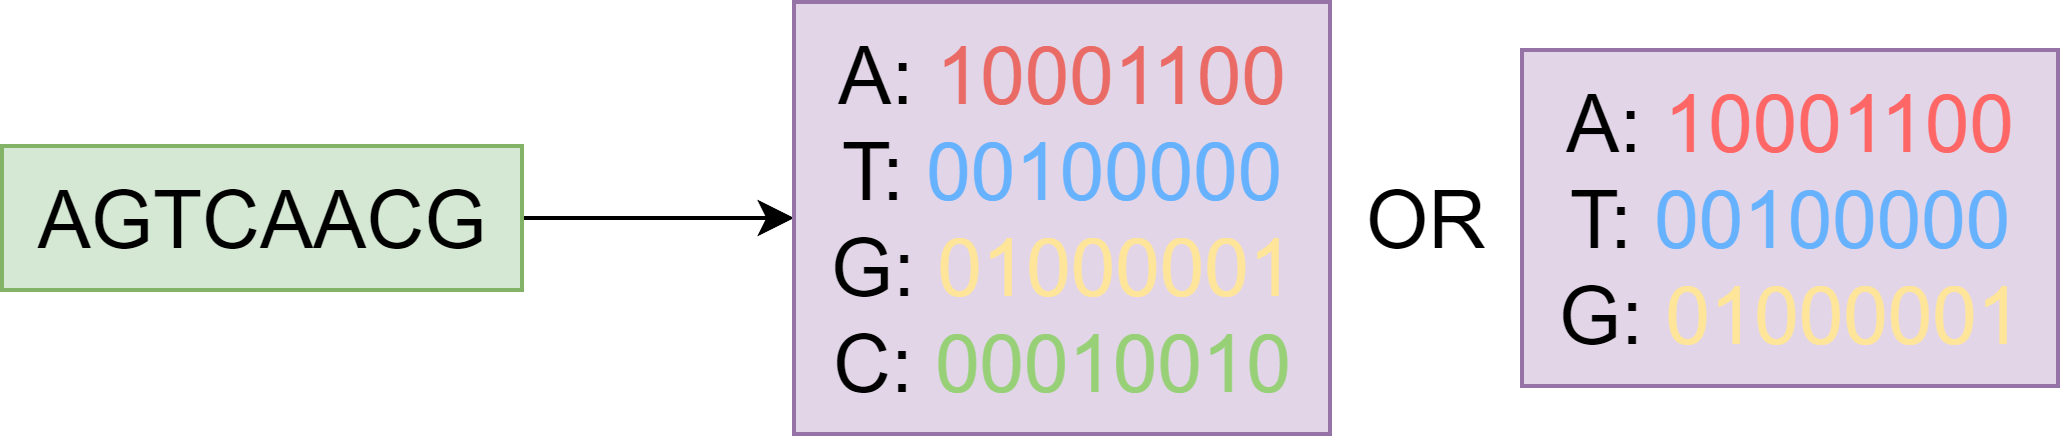
\includegraphics[width=0.6\textwidth]{dissertation-one-hot-encoding.png}
    \caption{One-Hot Encoding of Target Sequence}
    \label{fig:one-hot-encoding}
\end{figure}

With this in mind, we can now start the introduction of the machine learning methods developed for predicting the outcomes of prime editing.

\subsubsection{DeepPE}

Developed by Kim et al, DeepPE is one of the earliest attempt at predicting the outcomes of prime editing using machine learning and illustrated many possible determinants of PE efficiency. Most of the determinants discovered in their study are still valid today, but the model itself is not as relevant in terms of performance due to the constraints in datasets at the time of their publication. The model is also very limited in terms of editing types supported, focusing on predicting the efficiency of G to C substitution at the position +5 nick site of the target sequence. 

After the users provided the target sequence to edit, the web tool will propose a number of pegRNA sequences and evaluate their efficiency using the DeepPE model. The 47-nt long target sequence and the 17 to 37nt RTT+PBS sequences, as well as 20 explicit features including the GC content and melting temperature of the PBS are used as input to the model. The two nucleotide sequences are one-hot encoded into four dimensional matrices as mentioned in section \ref{sec:embedding}. The two embedded sequences and the explicit features are then concatenated(stacked) together and fed into a convolutional neural network with 10 $3 \times 4$ filters. The output is pooled using a deep reinforcement learning model instead of a traditional pooling layer, and then input into a fully connected layer with 1000 units. The result is linearly transformed to the DeepPE prediction score, indicating the efficiency of the editing process on the target sequence using the provided PBS and RTT.

A sketch of the model architecture is shown in \autoref{fig:deeppe}.

\begin{figure}[ht]
    \centering
    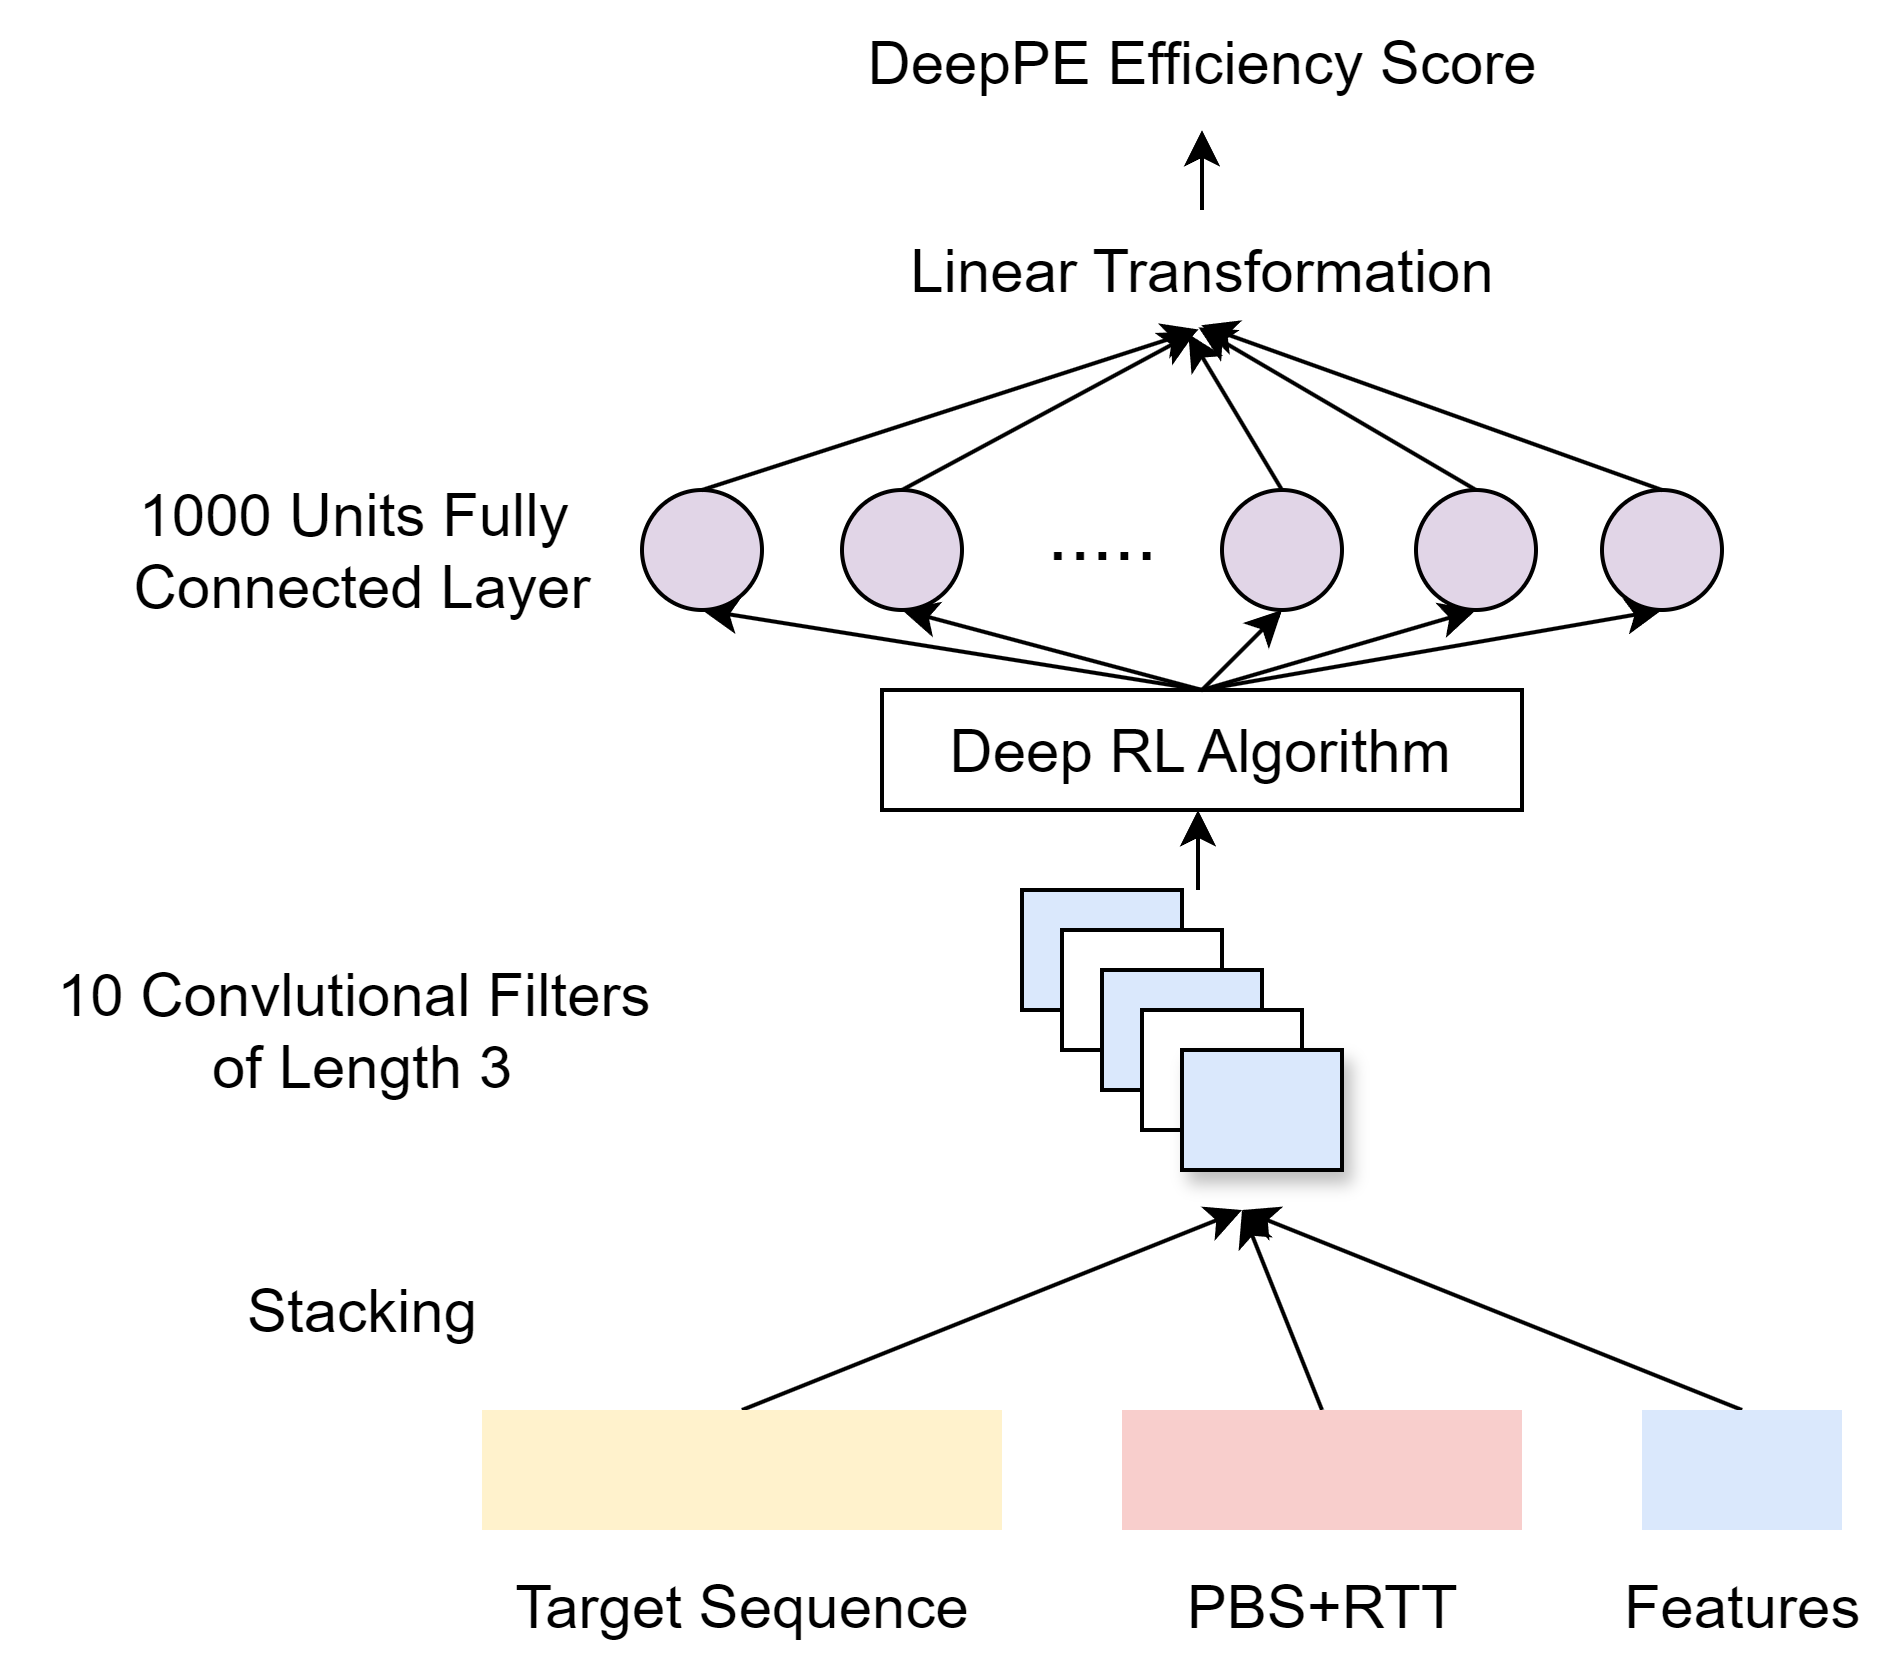
\includegraphics[width=0.55\textwidth]{DeepPE.png}
    \caption{DeepPE Model Architecture}
    \label{fig:deeppe}
\end{figure}

This architecture had the highest performance among the methods reviewed by the authors, although not significantly higher than L1 Lasso regression model. The model achieved a Spearman's R of 0.7 to 0.8, and a Pearson's r of 0.6 to 0.7 on the held-out as well as generalization(unseen) datasets.

The authors also developed another multi-layer perceptron(MLP) model to predict the editing efficiency of more general editing types, including single-nucleotide insertions, deletions and substitutions. However, random forest achieved better performances and was thus used in the additional PE\_Type and PE\_Position models. PE\_Type model proposes pegRNA for 24 possible edits, including specific single-nucleotide deletions, insertions, and substitutions at designated locations. PE\_Position model proposes pegRNA optimized to perform substitutions at ten more positions, namely positions 1, 2, 3, 4, 6, 7, 8, 9, 11 and 14.

\subsubsection{Easy Prime}

EasyPrime is a XGBoost regression model developed by Liu et al to produce design for RTT, PBS and ngRNA. Instead of arbitrary mutations, Easy-Prime predicts the editing efficiency of the variants logged in the Genome-Wide Association Studies(GWAS) database. The GWAS variants are the single nucleotide polymorphisms(SNPs) that have been associated with particular traits or diseases.

Similar to DeepPE, for each variant, the web tool proposes a number of pegRNA design using the constrains on PBS, RTT and ngRNA length provided by the user. The proposed pegRNAs are then evaluated by the XGBoost models to find the optimal candidate. When producing the efficiency score, EasyPrime takes the extracted features from pegRNA and target sequences as input to the model instead of the sequences themselves. The extracted features include GC content of the PBS, PAM sequence disruption, as well as several target mutation features describing the mutations to insert.

Cas9 activity score produced by DeepSpCas9 is also used as a feature in the model. DeepSpCas9 is a convolutional neural network model that predicts the activity of the SpCas9 protein on a given target sequence and sgRNA pair. The model architecture is very similar to DeepPE, with one convolutional layer followed by three fully connected layers. The unique feature of the model is the use of filters of different sizes in the convolutional layer(3, 5, and 7nt), allowing the model to capture the dependencies between the base pairs at different distances\cite{kimSpCas9ActivityPrediction2019}.

Albeit limited in the type of edits supported, EasyPrime is one of a few methods that provides official support for ngRNA design required by PE3 and PE3b. Note that PE3b is the optimized version of PE3, where the ngRNA is selected to avoid possible DSB by not targeting the nucleotide complementary to the nicked position\cite{liudavidr.SearchandreplaceGenomeEditing2019}.

Constrained by the data available and the simple architecture of the model, the performance of EasyPrime is relatively low compared to the other models reviewed. The model achieved a Spearman's R and Pearson's r of 0.5 to 0.6 on their held-out datasets.

\subsubsection{MinsePIE}

\label{sec:minsepie}

Koeppel et al. developed MinsePIE, a model that focuses on predicting the efficiency of insertions of varying lengths. It supported editing of cells with or without MMR deficiency, which can be interpreted as the result of using PE2 or PE4 with additional MLH1dn protein. 

The authors compared the performance of Lasso regression, Ridge regression, Random Forest, XGBoost regression, and a MLP model with hidden layers of size $(1000, 100)$. The Gradient Boosting model with the XGBoost library achieved the best performance, and was thus selected as the final model. 

The web tool works nearly identically to DeepPrime, with the additional constraint in homology arm length. The sequence to insert is surrounded by curly brackets inside of the target sequence. The user can also explicitly define a set of PBS, RTT and spacer, omitting the step of the web interface proposing candidate pegRNA for the model to evaluate. 

It also only takes ten extracted features as input to the model instead of the one-hot encoded sequences. This significantly reduces the computational cost of the model, as the one-hot encoding of the sequences can be very large for long sequences. On the other hand, it also limits the model's ability to capture certain unknown features that are present in the sequences. This resulted in a relatively weaker performance compared to the other models published around the same time(DeepPrime, PRIDICT). However, with the significantly larger training datasets, it still outperformed EasyPrime designed with a similar architecture.

The final model trained on the full training set achieved a correlation of 0.68 on held-out sequences, with performance ranging from R = 0.44 to 0.92 when restricted to datasets from individual screens.

\subsubsection{DeepPrime}

\begin{figure}[ht]
    \centering
    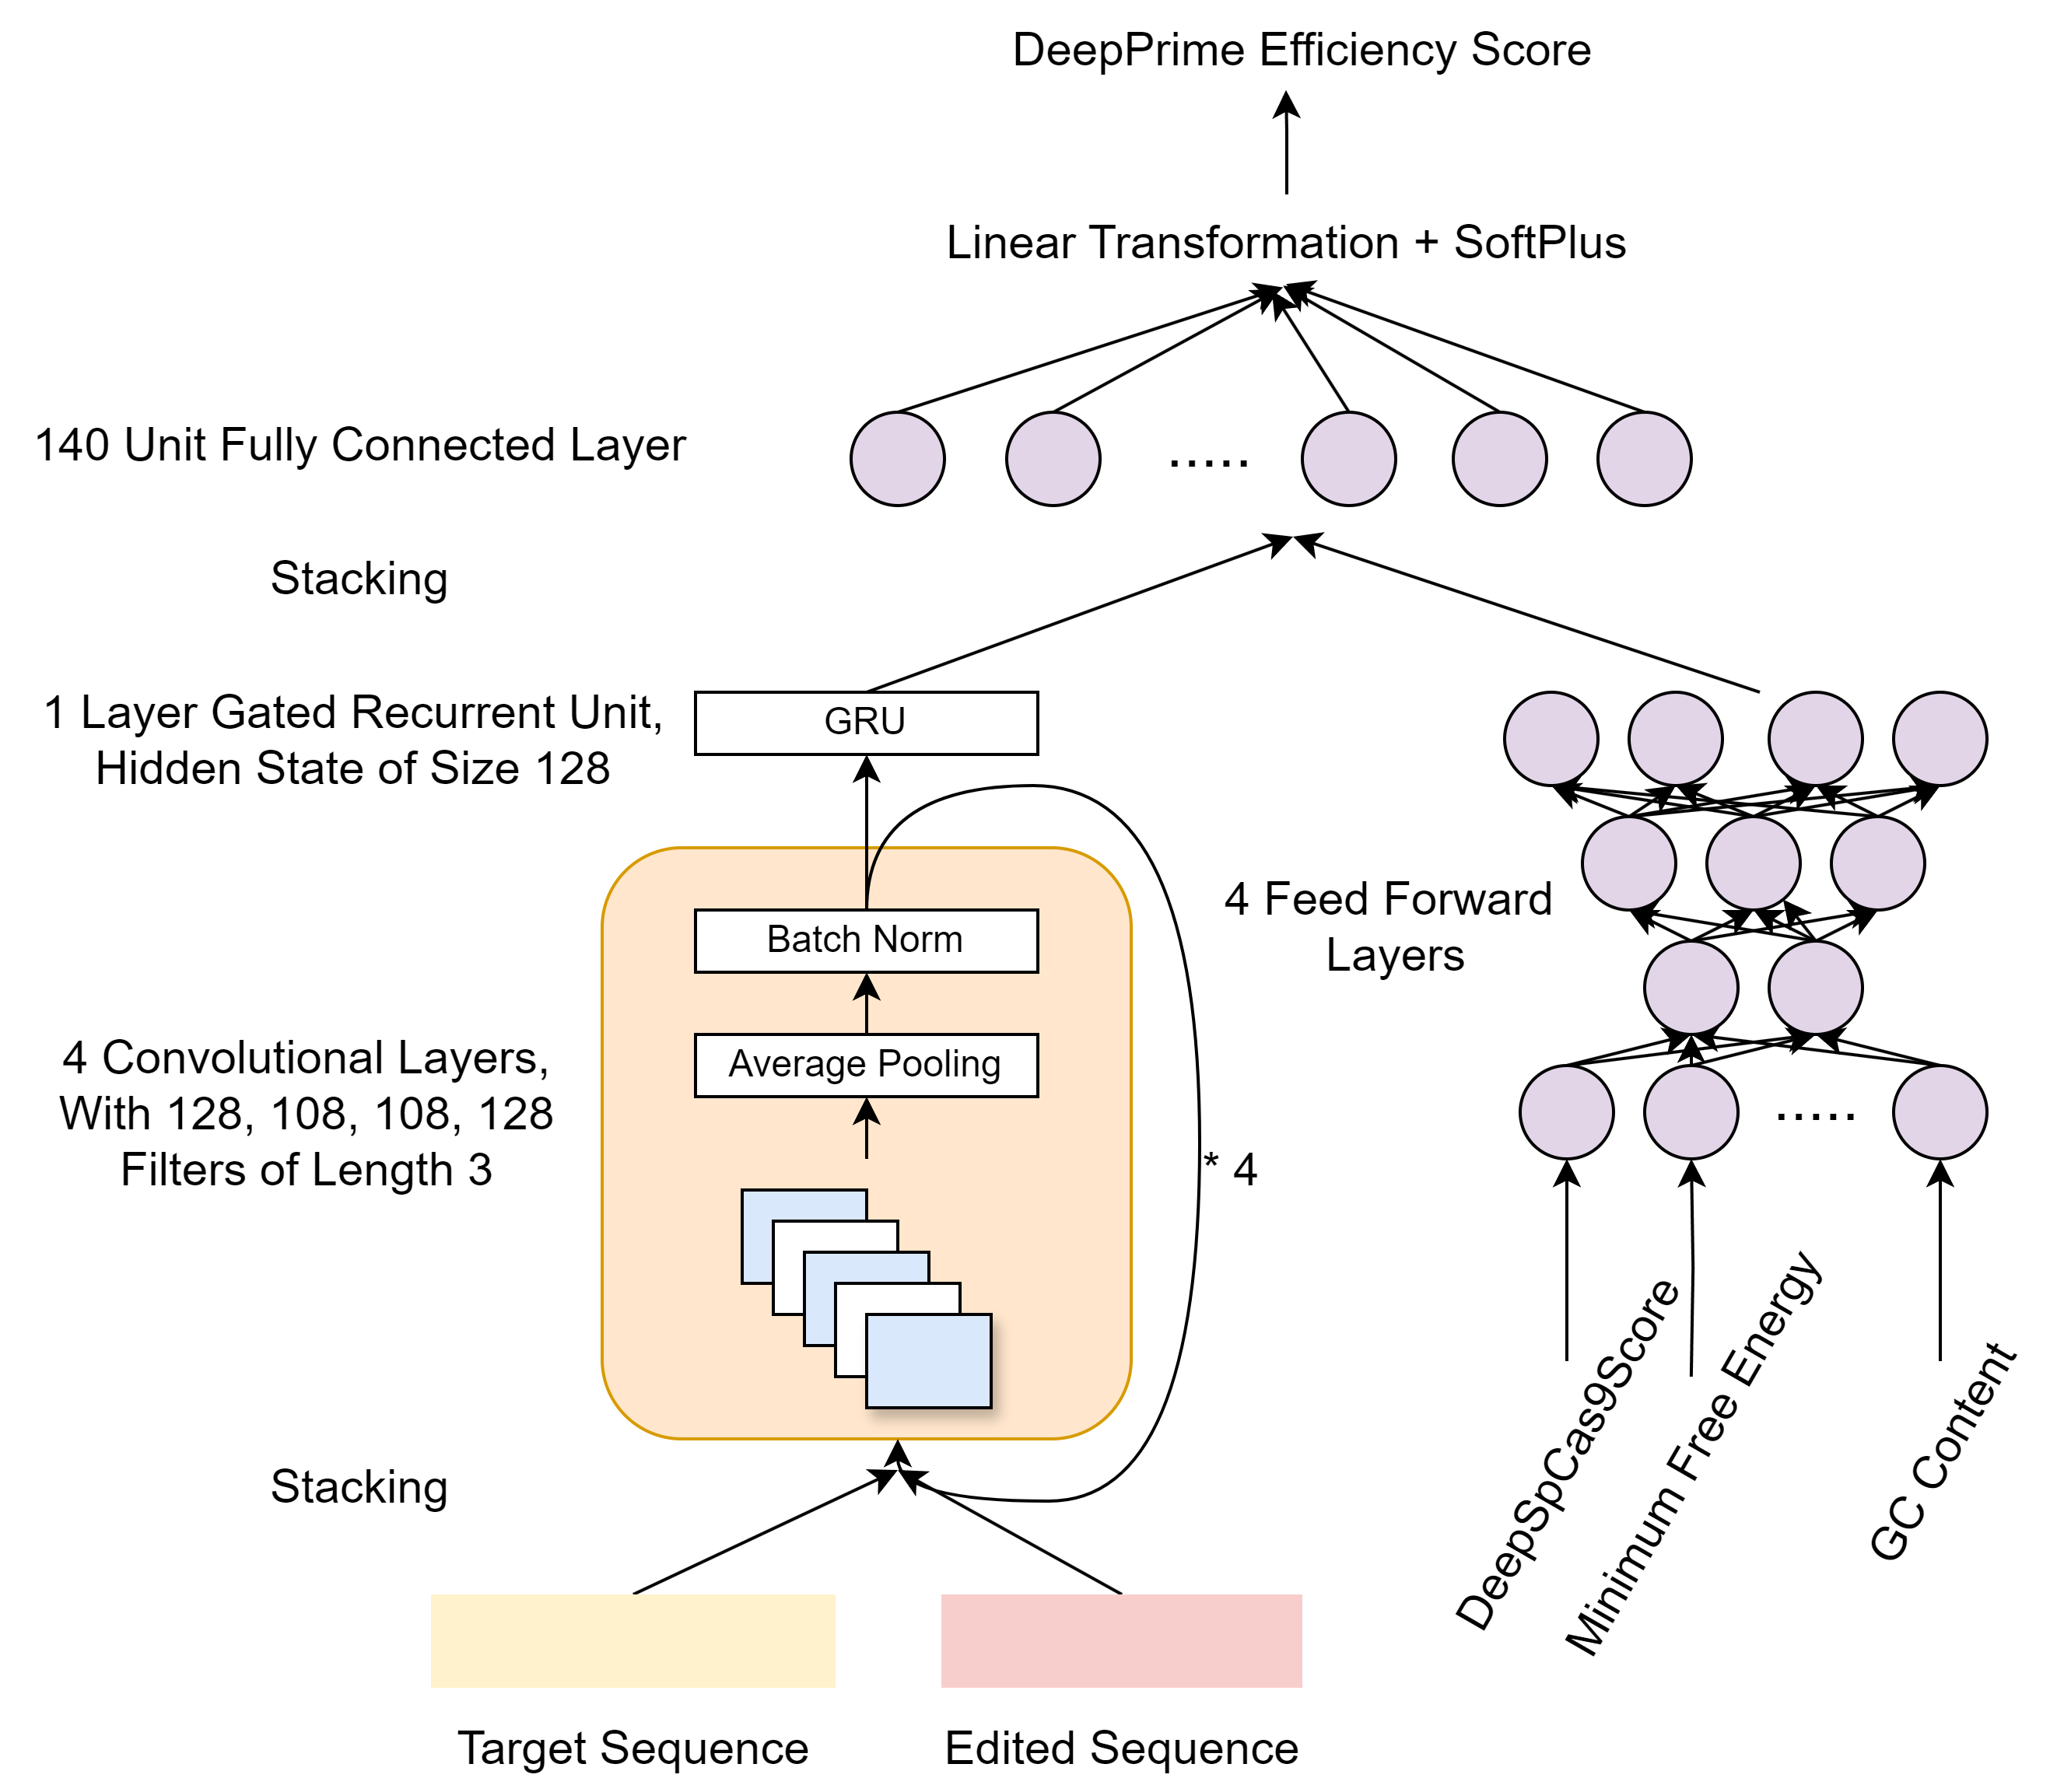
\includegraphics[width=0.8\textwidth]{DeepPrime.png}
    \caption{DeepPrime Model Architecture}
    \label{fig:deepprime}
\end{figure}


Also developed by Kim et al., DeepPrime is the updated version of DeepPE with an upgraded model architecture. 

Illustrated in \autoref{fig:deepprime}, instead of PBS + RTT with target sequence, it takes the wild type(unedited) as well as the edited sequences as input to the CNN. The convolutional network is significantly larger than DeepPE, containing four convolutional layers with 128, 108, 108, and 128 filters, respectively. Moreover, conventional average pooling is used this time round after each convolutional layer instead of a deep RL algorithm. Batch normalization is also applied to accelerate training.  The output of the convolutional layer is then processed by bidirectional Gated Recurrent Units(GRU). 

Instead of processed together with the embedded sequence, features extracted from the proposed pegRNA and target context sequence are processed using a separate four-layer feed forward neural network. The outputs from the two networks are then stacked and fed into a fully connected layer. The result is linearly transformed and processed by a SoftPlus activation function to produce the final prediction score.


DeepPrime is effectively a multi-task learning model, with a base model trained using the combination of 18 datasets of different PE and cell line combinations. The base model is then fine tuned using each of the 18 datasets to produce a task specific model for each setting, collectively named DeepPrime-FT.  

Shown in \autoref{tab:ml-methods}, the max PEs(PE2max, PE4max) are the versions with updated reverse transcriptase and SpCas9 nickase. epegRNAs(engineered pegRNAs) are pegRNAs with additional $3'$ RNA structural motif that increases prime editing efficiency\cite{chenEnhancedPrimeEditing2021}. NRCH-PEs are PEs that supports the additional NRCH PAM.

The amount of training data used makes DeepPrime the most comprehensive method in terms of the number of cell lines and PE versions covered. At the same time, the multi-task design allows DeepPrime-FT to utilize the share features between the different PEs and cell lines, and thus achieve very high performance. 

The model has made significant improvement compared to DeepPE, with a Spearman's R of 0.8 to 0.9, and a Pearson's r of 0.7 to 0.9 on most of the testing datasets, including the generalization datasets unseen during training.

\subsubsection{PRIDICT}

\begin{figure}[ht]
    \centering
    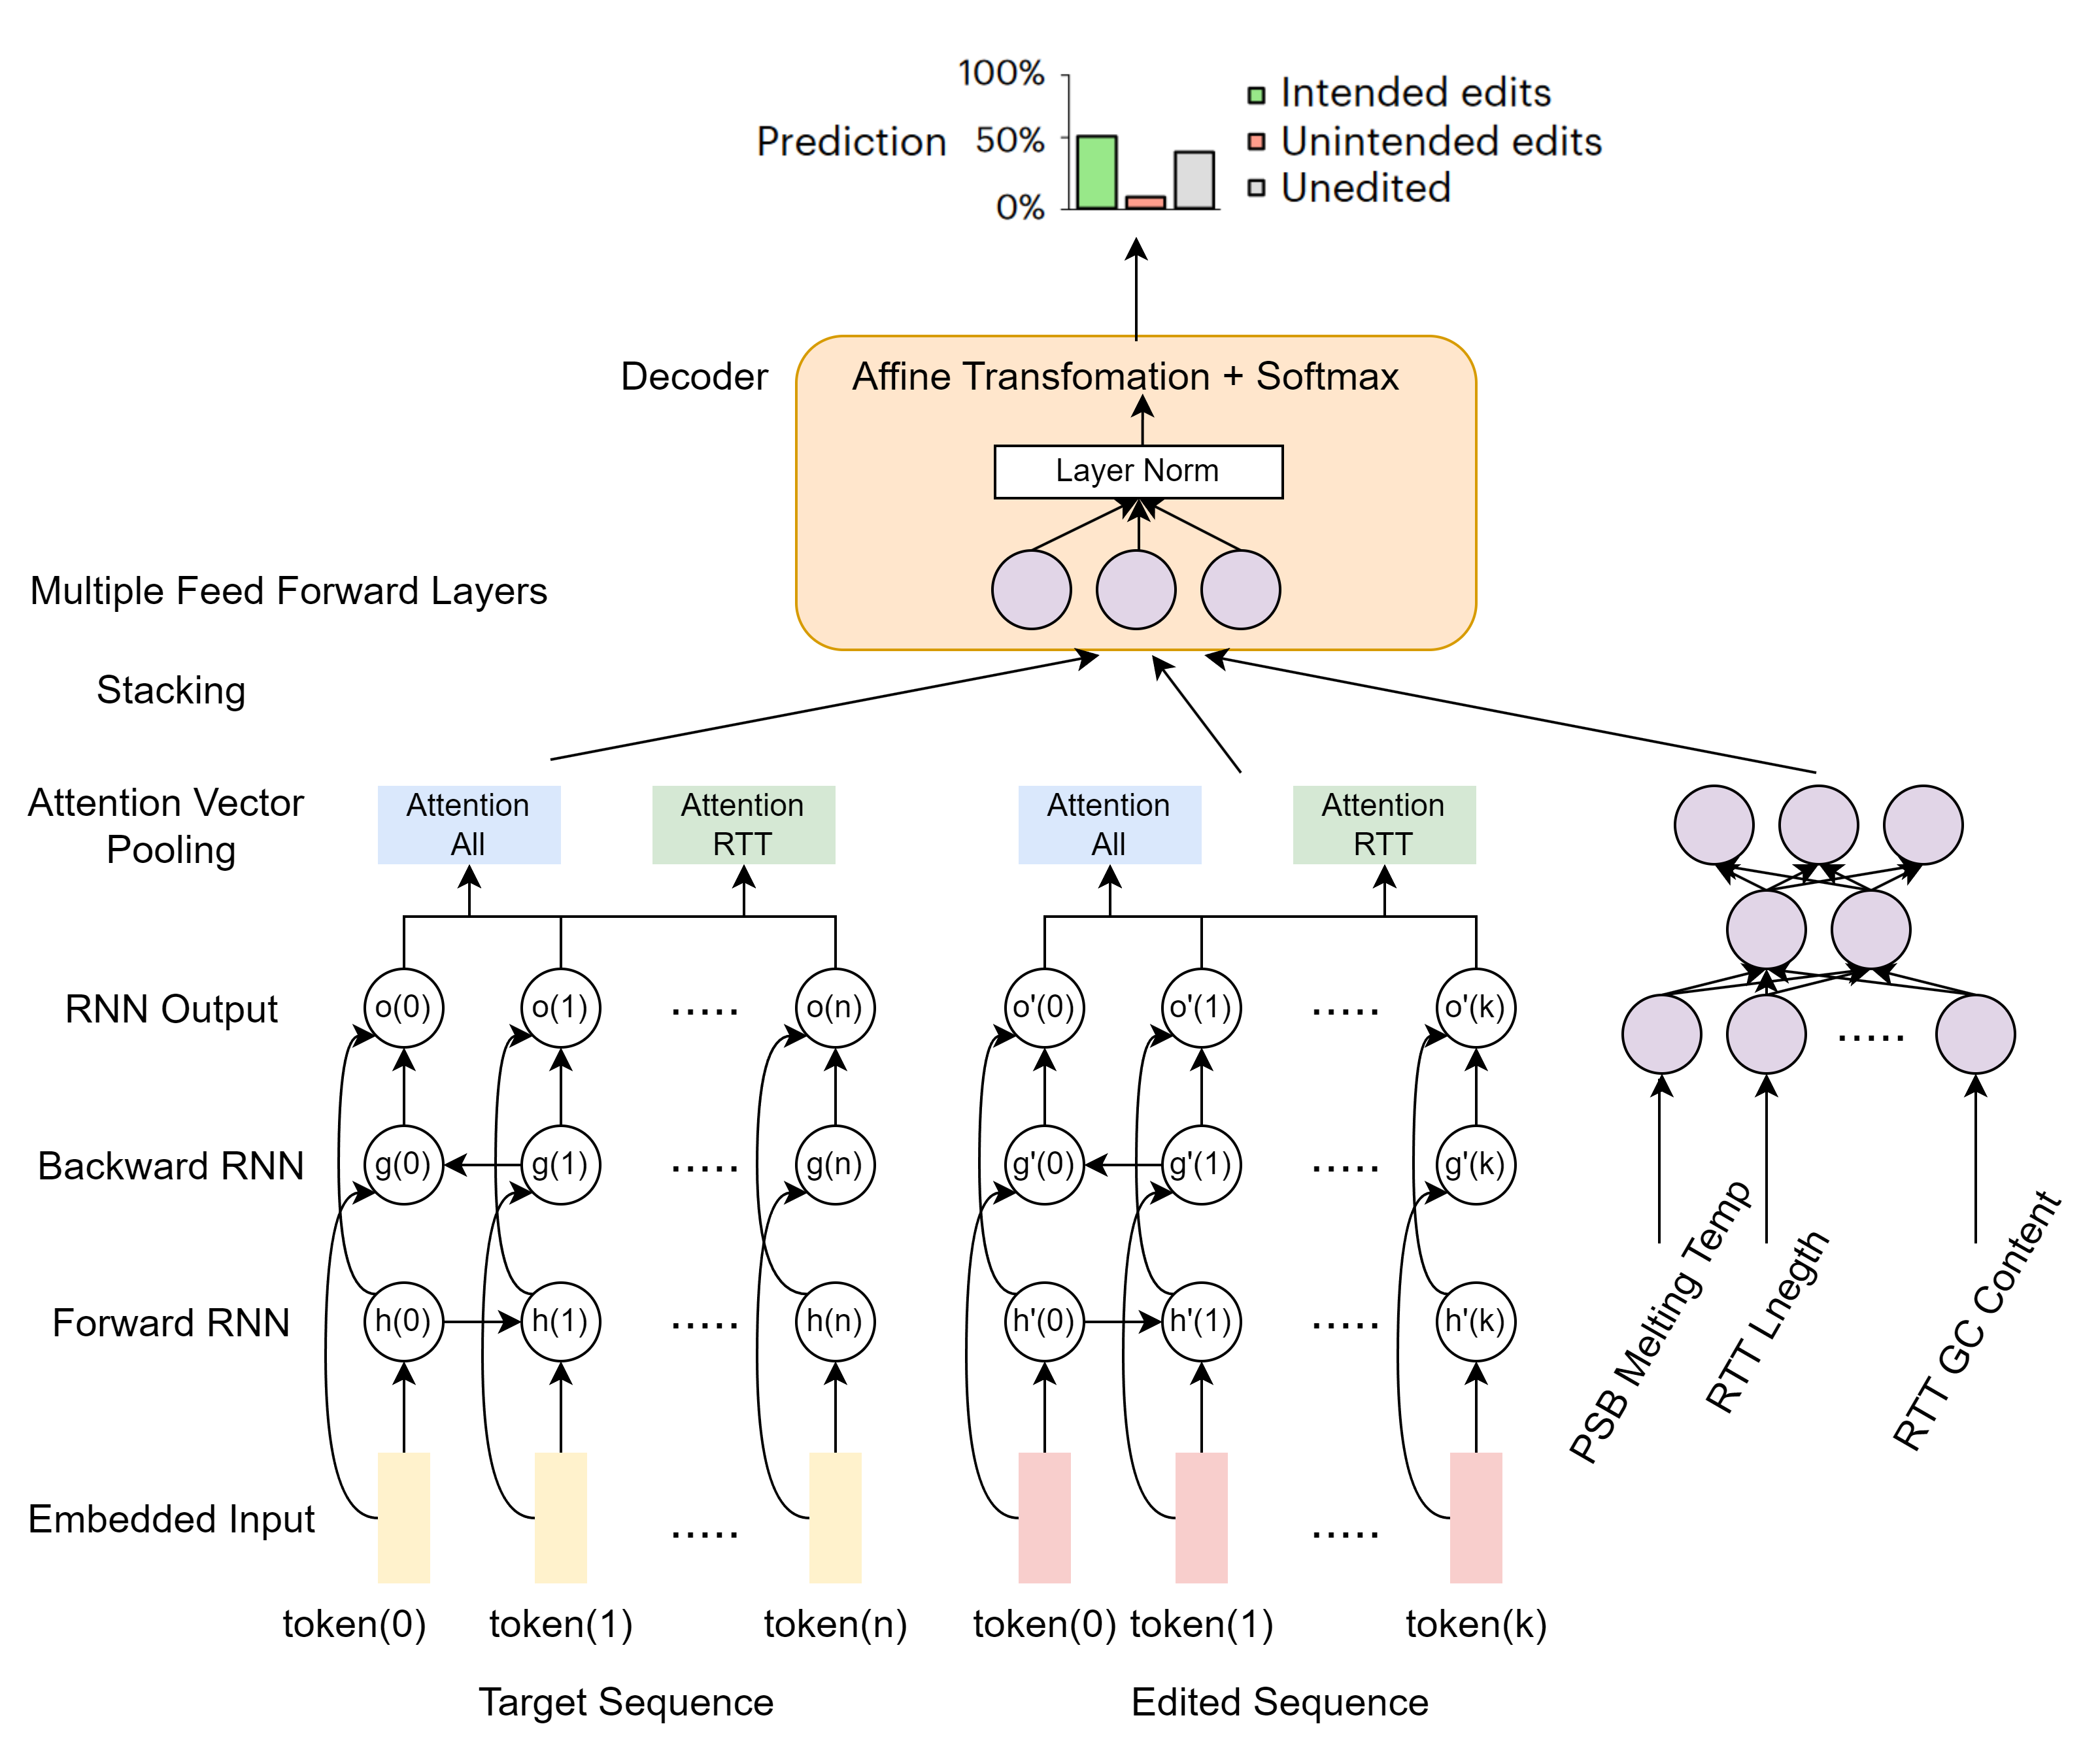
\includegraphics[width=\textwidth]{pridict.png}
    \caption{PRIDICT Model Architecture\cite{mathisPredictingPrimeEditing2023}}
    \label{fig:pridict}
\end{figure}


Developed by Gerald Schwank et al, PRIDICT utilizes a sophisticated attention-based bidirectional RNN model with a similar pegRNA recommendation pipeline to DeepPE and DeepPrime. 

The model overall is a three encoder one decoder architecture. Two of the encoders are attention-based bidirectional RNN models, learning the vector representation of the sequence data. The third encoder is a feed forward neural network taking explicit features derived from the proposed pegRNA, such as the length of the modifications to insert and melting temperature of the PBS, as inputs, similar to DeepPrime.

The target and mutation sequences are one-hot encoded as described in section \ref{sec:embedding}, alongside three additional binary encoding indicating whether the nucleotide belongs to the protospacer, RTT or PBS. The four embeddings are stacked together into a vector of length 9 for each token in the target sequence and 7 for the mutated sequence(the protospacer embedding is omitted for mutated sequence) and fed into the model.

The bidirectional RNN model is used to capture the dependencies between the base pairs within the whole sequence, instead of only past information captured by unidirectional RNN models. Two separate attention query vectors then pools(compresses) sequence of token-level representations into one fixed length vector using the calculated attention weights. One query vector pools all tokens of the sequences, providing context. The other pools only RTT tokens, focusing on the part where the edits are made. 

The decoder is another feed forward neural network with residual connections and layer normalization, taking the pooled vectors from the encoders and calculating the probability distribution of possible outcomes of the edits when using the proposed guide. 

The model architecture is illustrated in \autoref{fig:pridict}.

Significantly higher performance was achieved by PRIDICT when compared to DeepPE (including PE\_Type and PE\_Position) and EasyPrime, with 2-3 fold increase in Spearman's R and Pearson's r on the generalization datasets curated by Gerald et al. PRIDICT also achieved comparable or better results on the datasets DeepPE and EasyPrime were originally trained on. In terms of current generation of models, it was on par with DeepPrime on the HEK293T datasets when predicting intended edits, with a Spearman's R of 0.81. At the same time, PRIDICT outperformed the MinsePIE model as mentioned in section \ref{sec:minsepie}.


\section{Discussion}

A clear increasing trend in the performance of the models as well as the size and variety of the datasets can be observed over the years. DeepPrime supports an enormous amount of prime editors and cell types, while PRIDICT shows very high and consistent performance across different datasets. Limits on editing types are also being pushed, from the simple G to C substitution in DeepPE to arbitrary edits supported by PRIDICT and EasyPrime.

However, many improvements can still be made to further advance the field.

\subsection{Future Directions}


\subsubsection{Incoorperation of Advanced Tokenizer}

First of the possible directions is the possibility of using a newly emerged tokenizer instead of one-hot encoding during data embedding. Chen et al proposed a `fingerprinting' tokenization method that can capture the essential of RNA-DNA hybrids in Cas9 system. It had been shown to improve the performance of machine learning systems including XGBoost classifiers in the task of predicting the efficiency of CRISPR-Cas9 HDR\cite{chenGenomewideCRISPROfftarget2023}. 

The method can potentially be applied to the aforementioned prime editing models, as the RNA-DNA hybrid is also a crucial part of the prime editing process. 

\subsubsection{Application of Other Advanced Model Architecture}

State of the art model architectures including the transformer can also be applied to the task. Transformer has shown to be very effective in capturing the dependencies between the base pairs in the sequence, and has been applied to the task of predicting base editing efficiency with great success, outperforming RNN and CNN\cite{marquartPredictingBaseEditing2021}. As a result, the model can potentially be applied to the task of predicting prime editing efficiency as well. 

\subsubsection{Using Ensemble Learning to Improve Overall Accuracy}

Moreover, more than one models can be utilized at the same time during pegRNA design. As discussed in section \ref{sec:ml-methods}, each model has its own features and design choices, resulting in individual limitations and advantages. Ensemble learning is a technique used to mitigate errors or biases that may exist in individual models by leveraging the collective intelligence of the ensemble, and possibly result in a more accurate and robust model.

\subsubsection{Development of Benchmarking Datasets}

At the same time, it was very difficult to directly gauge the performance of the models due to the lack of a consistent benchmarking dataset during the survey. To validate whether their methods produced significant improvements, the authors had to train and test all previous representative models on their own datasets. This is feasible at the current stage of the field, but as the number of models and datasets grow, it will become increasingly difficult to compare the performance of the models. 

A benchmarking dataset can be curated for each PE and cell line combination, and the studies can include the performance of the models on the relevant datasets in their publications. This will allow for a more direct comparison of the models and provide a clearer picture of the current state of the field.


\newpage

\printbibliography

\end{document}
